
% this file is called up by thesis.tex
% content in this file will be fed into the main document

%: ----------------------- introduction file header -----------------------
\chapter{Related Work}\label{ch:soa}

\graphicspath{{soa/figures/}}

% -------------------------------------------------------------
% -- Related Work
% -------------------------------------------------------------

Recent studies \cite{Westergaard2017}\cite{Sciences2016} have shown that text mining of full research articles give consistently better results than using only their corresponding abstracts. Given the size limitations and concise nature of abstracts, they often omit descriptions or results that are considered to be less relevant but still are important in certain Information Retrieval (IR) tasks. Thus, when other researchers cite a particular paper, 20\% of the keywords that they mention are not present in the abstract \cite{Divoli2012}.



\section{Text Annotations}
% https://onnx.ai/

The annotation of human-readable documents is a well-known problem in the Artificial Intelligence domain in general and Information Retrieval and Natural Language Processing fields in particular. There already exist a broad set of tools and frameworks able to analyze text for automatically producing such annotations, at very different levels of granularity: from minimal units such as terms and entities, to descriptors at the level of the entire collection such as  topics or summaries. For example, StanfordNLP~\cite{Manning2014TheToolkit} framework allows to perform different operations such as Part-of-Speech (PoS) tagging or Named Entity Recognition in various languages. Others like Mallet\footnote{\url{http://mallet.cs.umass.edu}} or SparkLDA\footnote{\url{https://spark.apache.org/mllib/}} perform topic modeling and clustering. We are focused on the transversal problem of making those standalone tools coexisting under the same solution. Being able to effectively integrating  them  under a common ecosystem helps to seamlessly obtain different kind of  annotations and boost the way those solutions can make sense of document collections.  
 
Certain systems among the research and industrial communities have already integrated some of the annotation tools introduced above. For example, \cite{gate2013} works with records from the biomedical domain, where robustness and high precision are prioritized. Therefore they rely on techniques supported by  GATE\footnote{\url{https://gate.ac.uk/}} framework, which widely supports hand-crafted, domain specific techniques such as rules or finite state transducers. On the other side of the spectrum we find \cite{chielang2012}, where the authors try to annotate text from a much noisier, sparser and error-prone medium: a tweet stream. Therefore they do not rely on any linguistic feature, due to the unpredictable way short social media post are written. We observe how each of those examples has very specific needs and leverages on certain annotation tools in order to accomplish the tasks it was originally created for. In both systems the involved components are highly coupled so they can not be easily extended to contemplate complementary annotation tools or alternative modules. 
%On the contrary, \textit{librAIry} advocates loosely interconnected components that make the architecture more reusable and expandable in other systems across domains.
 
One crucial problem regarding the re-usability and expansion possibilities of those systems and the tools they leverage on is the language they have been developed in. For example, Mallet uses Java, but others like spaCy \footnote{\url{https://spacy.io}} are python-based. To the best of our knowledge, there has not been any significant efforts on reconciling into a single architecture such heterogeneous set of tools, therefore minimizing the engineering effort and maximizing scalability of the system so it can be applied to very different domains and textual annotation tasks.

In addition, available annotation systems rely on certain storage solutions that are suited for some tasks but are less adequate others. For example \cite{furlong2008osirisv1} uses a relational database (MySQL\footnote{\url{https://www.mysql.com/}}) to ensure reliability and speed in managing the indexed information. In \cite{rizzo20153cixty},  the authors leverage on Virtuoso triple-store to provide native graph operations over the data. But new requirements may be considered for those systems so different storage needs can come into play.  For example, column oriented databases (Cassandra\footnote{\url{http://cassandra.apache.org}}) can help to better handle high-volume queries on specific data fields. Same goes with text oriented indexes such as ElasticSearch \footnote{\url{https://www.elastic.co}}, which can provide customized text-based search operations over the available information. 
%\textit{librAIry} straightforward supports the coexistence of different storage solutions, so it can be agnostic to the kind of underlying storage modules implemented. Thanks to the distributed nature of the proposed architecture,  different databases can be synchronized under the same common environment working together to store and deliver results in a more efficient manner.


\section{Topic-based Relations}

Traditional retrieval tasks over large collections of textual documents \cite{Hearst1999} highly rely on individual features like term frequencies (e.g. TF-IDF). However, new ways of characterizing documents based on the automatic generation of models surfacing the main subjects covered in the corpus have been developed during recent years. Probabilistic Topic Modeling \cite{Blei2010} algorithms are statistical methods that analyze the words of the original texts to discover the themes that run through them, how those themes are connected to each other, or how they change over time.

Probabilistic topic models do not require any prior annotations or labeling of the documents. The topics emerge, as hidden structures, from the analysis of the original texts. These structures are topics distributions, per-resource topic distributions or per-resource per-word topic assignments. In turn, a topic is a distribution over terms that is biased around those words associated to a single theme. This interpretable hidden structure annotates each resource in the collection and these annotations can be used to perform deeper analysis about relationships between resources. In this way, topic modeling provides an algorithmic solution to organize and annotate large collections of textual documents according to their topics.

The simplest generative topic model is \textit{Latent Dirichlet Allocation} (LDA) \cite{Blei2003}. This and other topic models such as \textit{Probabilistic Latent Semantic Analysis} (PLSA) \cite{Hofmann2001} are part of the field known as probabilistic modeling. They are well-known latent variable models for high dimensional data, such as the bag-of-words representation for textual data or any other count-based data representation. While LDA has roots in \textit{Latent Semantic Analysis} (LSA) \cite{Deerwester1990} and PLSA (it was proposed as a generalization of PLSA), it was also influenced by the generative Bayesian framework to avoid some of the over-fitting issues that were observed with PLSA.

This statistical model tries to capture the intuition that documents can exhibit multiple topics. Each document exhibits each topic in different proportion, and each word in each document is drawn from one of the topics, where the selected topic is chosen from the per-document distribution over topics. All the documents in the collection share the same set of topics, but each document exhibits these topics in a different proportion. Documents are represented as a vector of counts with $W$ components, where $W$ is the number of words in the vocabulary. Each document in the corpus is modeled as a mixture over $K$ topics, and each topic $k$ is a distribution over the vocabulary of $W$ words. Formally, a \textit{topic} is a multinomial distribution over words of a fixed vocabulary representing some concept. Each topic is drawn from a Dirichlet distribution with parameter $\beta$, while each document's mixture is sampled from a Dirichlet distribution with parameter $\alpha$. These two priors, $\alpha$ and $\beta$, are also known as hyper-parameters and they are estimated following some heuristic.

A Dirichlet distribution is a continuous multivariate probability distribution parameterized by a vector of positive reals whose elements sum to 1.  It is \textit{continuous} because the relative likelihood for a random variable to take on a given value is described by a probability density function, and also it is \textit{multivariate} because it has a list of variables with unknown values. In fact, the Dirichlet distribution is the conjugate prior of the categorical distribution and multinomial distribution.

Unlike a restrictive clustering model, where each document is assigned to one cluster, LDA allows documents to exhibit multiple topics. Moreover, since LDA is unsupervised, the topics covered in a set of documents are discovered from the own corpus; the mixed-membership assumptions lead to sharper estimates of word co-occurrence patterns.

\subsection{Distance Measures}
In a \textit{Topic Model} the feature vector is a topic distribution expressed as vector of probabilities. Taking into account this premise, the similarity between two topic-based resources will be based on the distance between their topic distributions, which can be also seen as two probability mass functions. A commonly used metric is the \textit{Kullback-Liebler} (KL) divergence. However, it presents two major problems: (1) when a topic distribution is zero, KL divergence is not defined and (2) it is not symmetric, which does not fit well with semantic similarity measures that are usually symmetric \cite{Rus2013}.

\textit{Jensen-Shannon} (JS) divergence \cite{Rao1982}\cite{Lin1991} solves these problems considering the average of the distributions as below \cite{Celikyilmaz2010}:

\begin{equation}
JS(p,q) = \sum\limits_{i=1}^K p_{i}*\log \frac{2*p_{i}}{p_{i}+q_{i}}  +  \sum\limits_{i=1}^K q_{i}*\log \frac{2*q_{i}}{q_{i}+p_{i}}
\label{eq:jsdivergence}
\end{equation}
where  $K$ is the number of topics and $p,q$ are the topics distributions

It can be transformed into a similarity measure as follows \cite{Dagan1998} :

\begin{equation}
sim_{JS}(D_i , D_j) = 10^{- JS(p,q)}
\label{eq:simjs}
\end{equation}
where  $D_i,D_j$ are the documents and $p,q$ the topic distributions of each of them.


\textit{Hellinger} (He) distance is also symmetric and is used along with JS divergence in various fields where a comparison between two probability distributions is required \cite{Blei2007a} \cite{Hall2008} \cite{Boyd-Graber2010}:

\begin{equation}
	He(p, q) = \frac{1}{\sqrt{2}}\cdot\sqrt{\sum\limits_{i=1}^K (\sqrt{p_i} - \sqrt{q_i})^2)}
	\label{eq:hedistance}
\end{equation}

It can be transformed into a similarity measure by subtracting it from 1 \cite{Rus2013} such that a zero distance means max. similarity score and vice versa:

\begin{equation}
	sim_{He}(D_i, D_j) = 1 - He(p,q)
	\label{eq:simhe}
\end{equation}

However, all these metrics are not well-defined distance metrics, that is, they do not satisfy triangle inequality \cite{Charikar2002}. This inequality considers $d(x, z) <= d(x, y) + d(y, z)$ for a metric $d$ \cite{Griffiths2007}. It places strong constraints on distance measures and on the locations of points in a space given a set of distances. As a metric axiom the triangle inequality must be satisfied in order to take advantage of the inferences that can be deduced from it. Thus, if similarity is assumed to be a monotonically decreasing function of distance, this inequality avoids the calculation of all pairs of similarities by considering that if $x$ is similar to $y$ and $y$ is similar to $z$, then $x$ must be similar to $z$. 

\text{S2JSD} was introduced by \cite{Endres2003} to satisfy the triangle inequality. It is the square root of two times the $JS$ divergence:

%S2JSD formula
\begin{equation}
    S2JSD(P,Q) = \sqrt{2*JS(P,Q)}
\label{eq:s2jsd}
\end{equation}


\section{Thematic Document Retrieval}


Making sense out of the similarity score is not easy. As shown in figure \ref{fig:topic_distances}, given a set of pairs of documents, their similarity scores vary according to the number of topics. So the distances between those pairs fluctuate from being more to less distant when changing the number of topics.
\begin{figure}

\begin{adjustbox}{minipage=0.45\linewidth,frame=1pt 5pt}
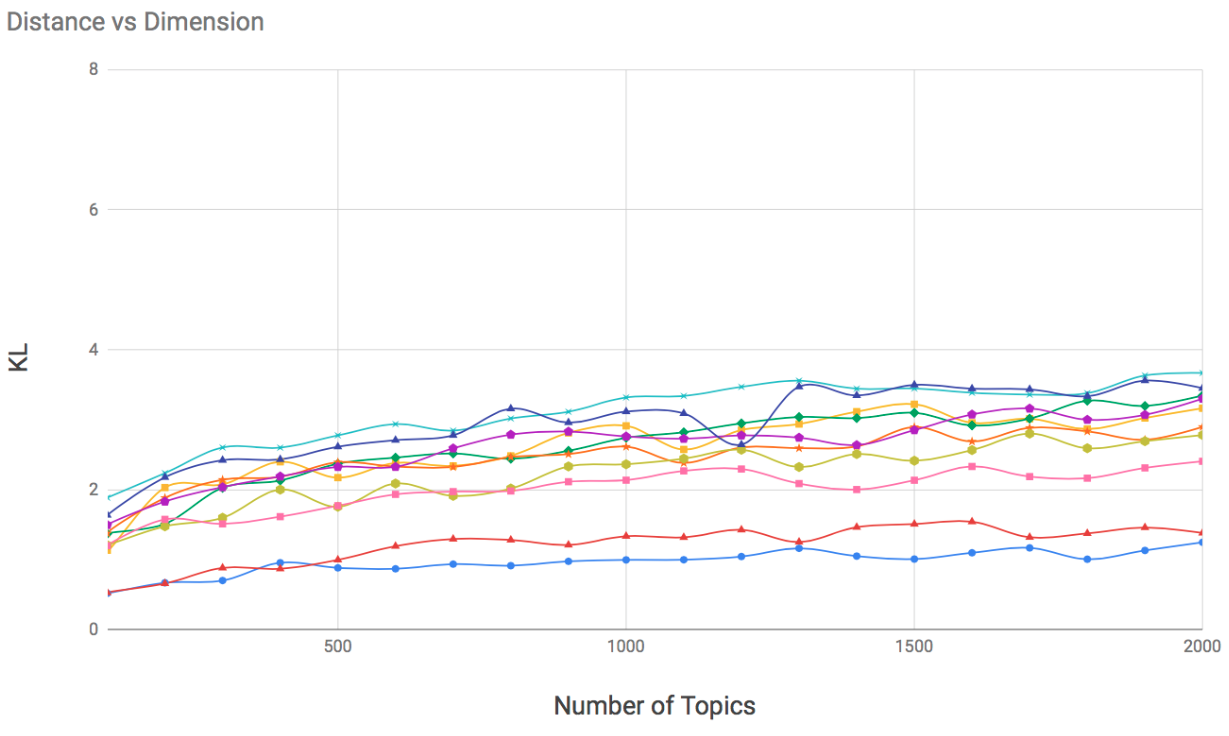
\includegraphics[width=\linewidth]{KL_100_2k.png}
\end{adjustbox}
\hfill
\begin{adjustbox}{minipage=0.45\linewidth,frame=1pt 5pt}
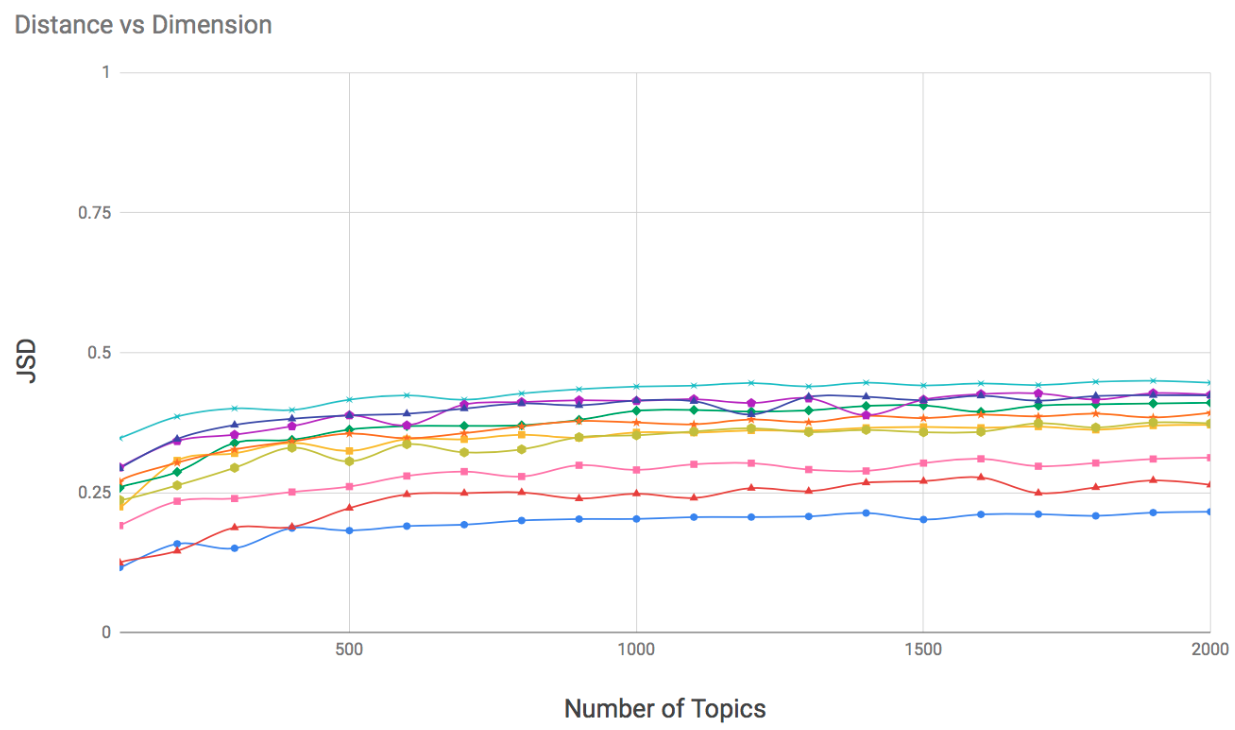
\includegraphics[width=\linewidth]{JSD_100_2k.png}
\end{adjustbox}
\hfill
\begin{adjustbox}{minipage=0.45\linewidth,frame=1pt 5pt}
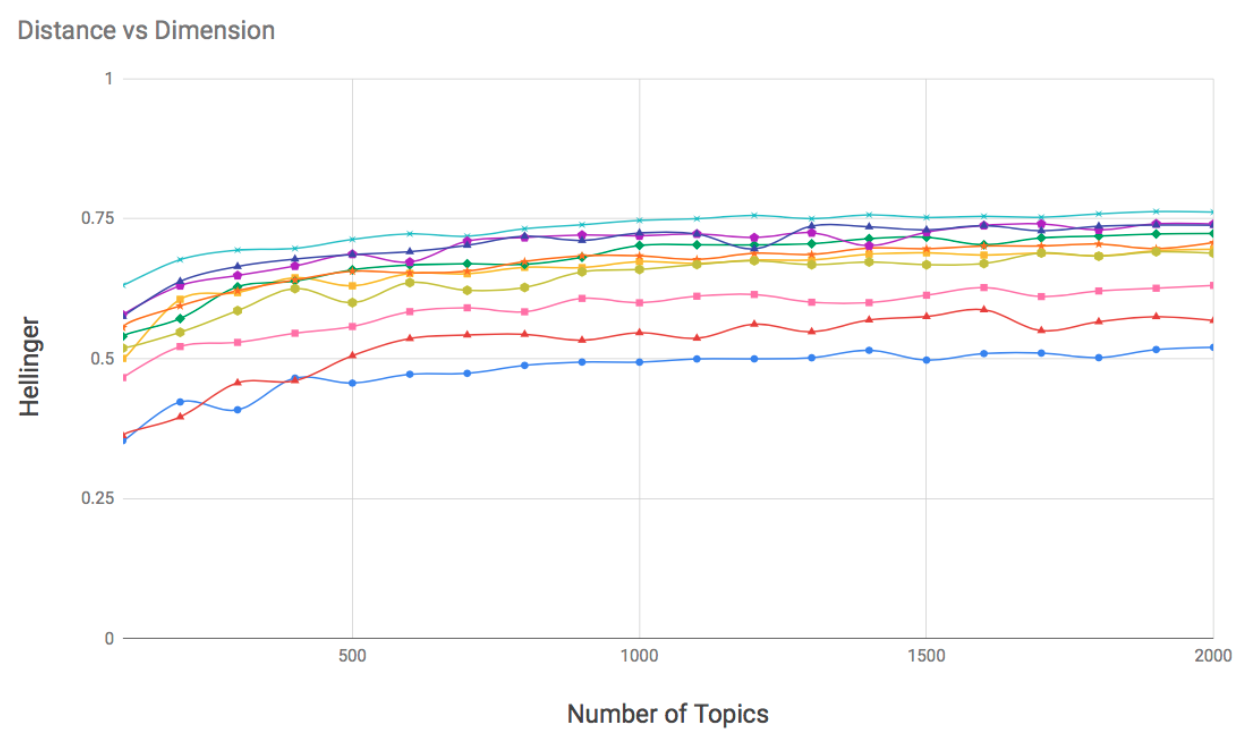
\includegraphics[width=\linewidth]{He_100_2k.png}
\end{adjustbox}
\hfill
\begin{adjustbox}{minipage=0.45\linewidth,frame=1pt 5pt}
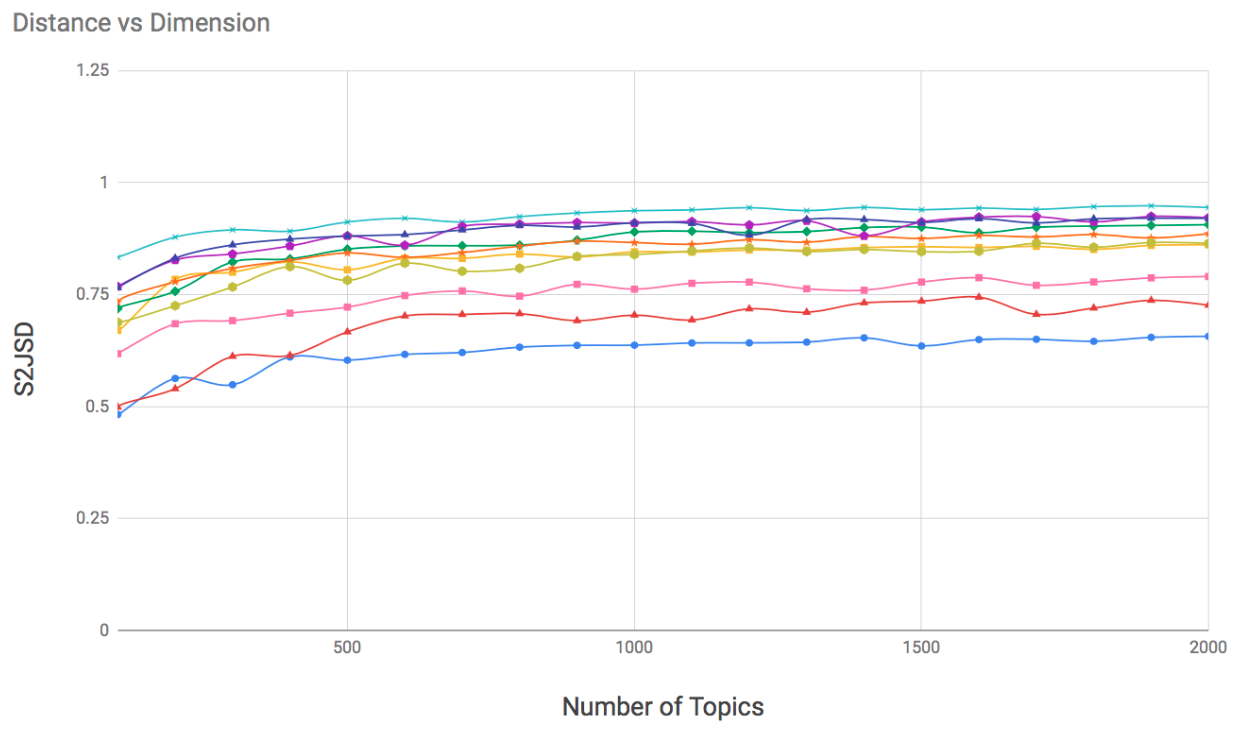
\includegraphics[width=\linewidth]{S2JSD_100_2k.png}
\end{adjustbox}
\caption{Distance values between 10 pair of documents from topic models with 100-to-2000 dimensions.}
\label{fig:topic_distances}
\end{figure}

Distances between documents generally increase as the number of dimensions of the space increases. This is due to the fact that as the number of topics describing the model increases, the more specific the topics will be. Topics shared by a pair of documents can be broken down into more specific topics that are not shared by those documents. Thus, similarity between pairs of documents is dependent on the model used to represent them when considering this type of metrics. We know that absolute distances between documents vary when we tune hyperparameters differently, but we also see that "relative distances" also change: e.g. for model M1, A is closer to B than C, but according to a M2 trained in the same corpora with different parameters , A is closer to C than B (cross-lines in fig \ref{fig:topic_distances}). This behaviour highlights the difficulty of establishing absolute similarity thresholds and the complexity to measure distances taking into account all dimensions. Distance thresholds should be model-dependent rather than general and metrics flexible enough to handle dimensional changes. 

These challenges have been tackled in this thesis by hashing methods based on clusters of topics to measure similarity, instead of directly using their weights. Hashing methods transform the data points from the original feature space into a binary-code Hamming space, where the similarities in the original space are preserved. They can learn hash functions (data-dependent) or use projections (data-independent) from the training data \cite{Wang2016}. Data-independent methods unlike data-dependent ones do not need to be re-calculated when data changes, i.e. adding or removing documents to the collection. Taking large-scale scenarios into account (e.g. Document clustering, Content-based Recommendation, Duplicate Detection), this is a key feature along with the ability to infer hash codes individually (for each document) rather than on a set of documents. 

Data-independent hashing methods depend on two key elements: (1) data type and (2) distance metric. For vector-type data, as introduced in section \ref{sec:similarity}, based on $l_p$ distance with $p \epsilon [0,2)$ lots of hashing methods have been proposed, such as p-stable Locality-Sensitive Hashing (LSH) \cite{Datar2004}, Leech lattice LSH \cite{Andoni2006}, Spherical LSH \cite{Terasawa2007}, and Beyond LSH \cite{Andoni2014}. Based on the $\theta$ distance many methods have been developed such as Kernel LSH \cite{Kulis2012} and Hyperplane hashing \cite{Vijayanarasimhan2014}. But only few methods handle density metrics in a simplex space. A first approach transformed the $He$ divergence into an Euclidean distance so that existing ANN techniques, such as LSH and k-d tree, could be applied \cite{Krstovski2013a}. But this solution does not consider the special attributions of probability distributions, such as Non-negative and Sum-equal-one. Recently, a hashing schema \cite{Mao2017} taking into account the symmetry has been proposed, non-negativity and triangle inequality features of the S2JSD metric for probability distributions. For set-type data, Jaccard Coefficient is the main metric used. Some examples are K-min Sketch \cite{Li2012}, Min-max hash \cite{Ji2013}, B-bit minwise hashing \cite{Li2010b} and Sim-min-hash \cite{Zhao2013}.

All of them have demonstrated efficiency in the search for similar documents, but none of them allows the search for documents (1) by thematic areas or (2) by similarity levels, nor they offer (3) an explanation about the similarity obtained beyond the vectors used to calculate it. Binary-hash codes drop a very precious information: the topic relevance.


\section{Multilingual Topic Alignment}

Multilingual probabilistic topic models (MuPTM) \cite{Vulic2015} have recently emerged as a group of language-independent generative machine learning models that can be used on large-volume theme-aligned multilingual text. Due to its generic language-independent nature and the power of inference on unseen documents, MuPTM's have found many interesting applications in many different cross-lingual tasks. They have been used on cross-lingual event clustering \cite{DeSmet2009}, document classification \cite{10.1007/978-3-642-20841-6_45} \cite{Ni:2011:CLT:1935826.1935887},  semantic similarity of words \cite{Mimno:2009:PTM:1699571.1699627}  \cite{Vulic:2012:DHC:2380816.2380872}, information retrieval \cite{10.1007/978-3-642-36973-5_9} \cite{ganguly-etal-2012-cross}, document matching \cite{Platt:2010:TDR:1870658.1870683} \cite{zhu-etal-2013-building}, and others. 

Once a PTM or MuPTM has been generated, documents can be represented by data points in a feature space based on topics to detect similarities among them exploiting inference results and using distance calculation metrics on it. Since exact similarity computations are unaffordable for neighbours detection tasks ($O(n^2)$), some algorithms based on approximate nearest neighbor (ANN) techniques have been proposed to efficiently perform document similarity search based on the low-dimensional latent space created by probabilistic topic models\cite{Zhen2016} \cite{Mao2017}. They transform data points from the original feature space into a hash-code space, so that similar data points have larger probability of collision (i.e. having the same hash code). However, the smaller space created by existing hashing methods lose the exploratory capabilities that topic models offer and the explanatory power that topics have to support the document similarity. The notion of topics is discarded and therefore the ability to make thematic explorations of documents. 

%Recently, a hashing algorithm that groups similar documents and preserves the notion of topics has been proposed \cite{Badenes-Olmedo2019}. It defines a hierarchical set-type data where each level of the hierarchy indicates the importance of the topic according to its distribution. Level 0 contains the topics of the document with the highest score. Level 1 contains the topics with highest score once the first ones have been eliminated, and so on. The knowledge provided by the topics to describe the documents is maintained and an efficient exploration of document collections on a large scale can be performed.

In this thesis we take PTM a step further, to make them cross-lingual through hierarchical representations created from a lexical data base. Documents from multi-language corpora are described by hierarchical expressions of multi-lingual concepts and can then be efficiently browsed and related without the need for translation. Hash codes are created from those concept hierarchies to perform document classification and information retrieval tasks on large document collections.
